i think we're finally getting towards finished hardware!

today is \textsc{if} amp work, because that's the last part that's being
persnickety. we need somewhere between 60 and 120 dB gain from the \lna to the
\adc, and we're doing our darnedest to get that. i made a preliminary design
that might get us close, but it's dependent on a lot of uncertain factors --
we'll have to see how it goes in real life.

\begin{figure}[H]
	\centering
	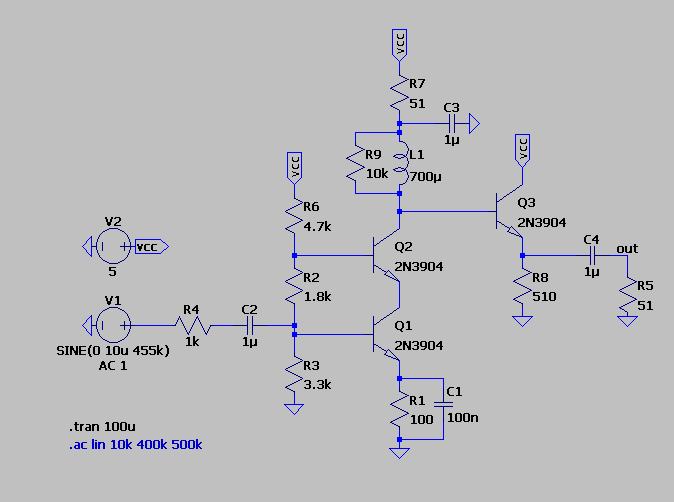
\includegraphics[width=0.7\textwidth]{if-amp-draft.png}
	\caption{my first draft for an amp; gives a little over 60 dB near 455
	kHz.}
\end{figure}

came up with a second draft, basically the same but with one fewer transistor.

\begin{figure}[H]
	\centering
	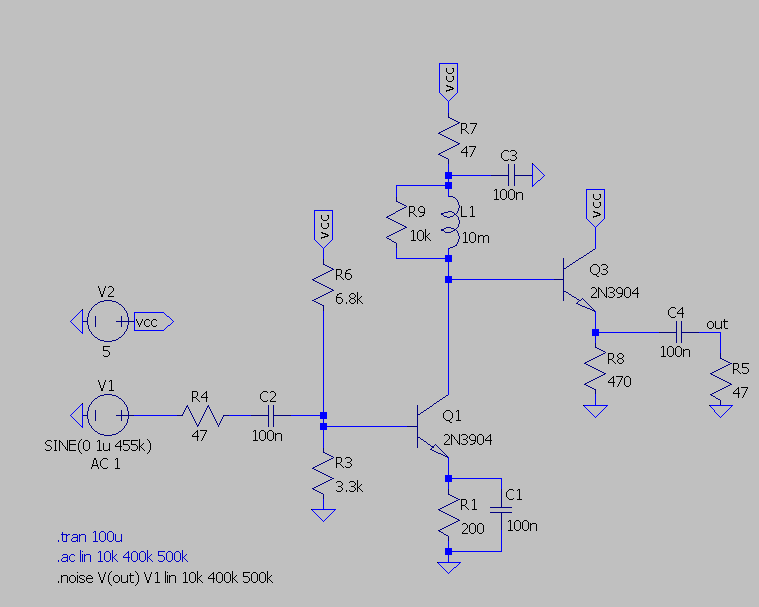
\includegraphics[width=0.7\textwidth]{if-amp-draft-2.png}
	\caption{same thing, basically.}
\end{figure}
